\section{Modelo de arquitectura de módulo}

El proyecto final (figura \ref{arquitectura}) fue diseñado como módulo de un AMS utilizado en universidades del estado de California.

\begin{figure}[]
\centering
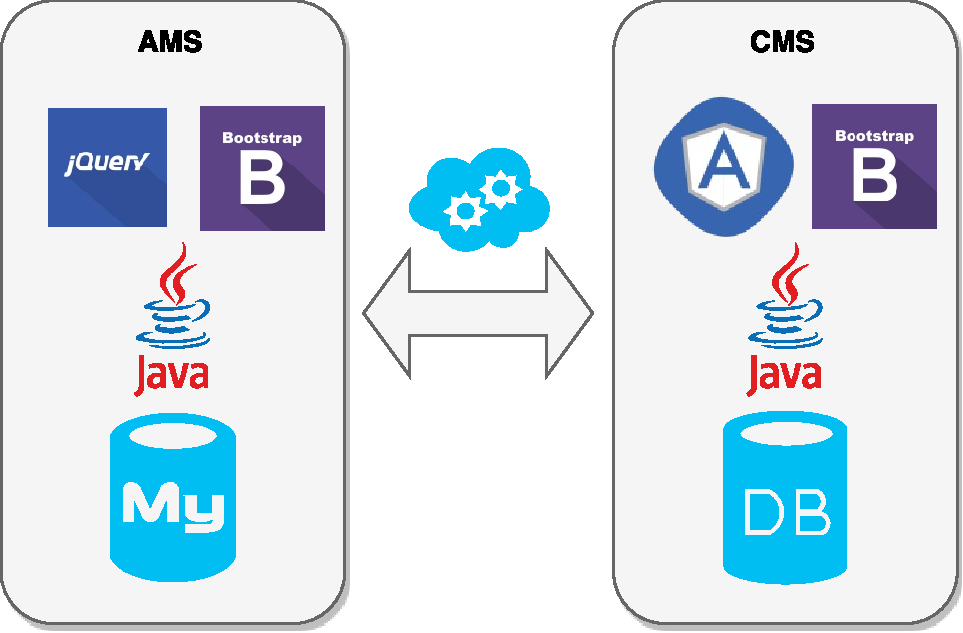
\includegraphics[scale=0.6]{Capitulos/PropuestadeSolucion/Imagenes/arquitectura}
\caption{Arquitectura del módulo curricular.}
  \label{arquitectura}
\end{figure}

El AMS utilizado como base tiene una trayectoria de largos años de uso en varias universidades. Utiliza MySQL como motor de base de datos, Java como lenguaje de programación para la lógica de la aplicación y como conector a la base de datos se utiliza, y Bootstrap y JQuery para la interfaz de usuario. 

El proyecto final va a utilizar la misma base de datos, lenguaje de programación, y Bootstrap como requisitos no funcionales para el módulo curricular. Se optó cambiar JQuery a AngularJS debido a que al contar con un modelo MVC\footnote{de sus siglas en inglés, Model View Controller, que significa en español modelo vista controlador.} en la capa de presentación desde el comienzo resultó muy atractivo para acelerar el ritmo de trabajo y poder comenzar a implementar interfaces más complejas sin tener que preocuparse por las cuestiones más triviales que Angular maneja con directivas ya definidas como el uso de \enquote{data binding}, además, cuenta con una cantidad de documentación de parte de la comunidad que lo hacía aún más atractivo.